% Options for packages loaded elsewhere
\PassOptionsToPackage{unicode}{hyperref}
\PassOptionsToPackage{hyphens}{url}
\PassOptionsToPackage{dvipsnames,svgnames,x11names}{xcolor}
%
\documentclass[
  letterpaper,
  DIV=11,
  numbers=noendperiod]{scrartcl}

\usepackage{amsmath,amssymb}
\usepackage{iftex}
\ifPDFTeX
  \usepackage[T1]{fontenc}
  \usepackage[utf8]{inputenc}
  \usepackage{textcomp} % provide euro and other symbols
\else % if luatex or xetex
  \usepackage{unicode-math}
  \defaultfontfeatures{Scale=MatchLowercase}
  \defaultfontfeatures[\rmfamily]{Ligatures=TeX,Scale=1}
\fi
\usepackage{lmodern}
\ifPDFTeX\else  
    % xetex/luatex font selection
\fi
% Use upquote if available, for straight quotes in verbatim environments
\IfFileExists{upquote.sty}{\usepackage{upquote}}{}
\IfFileExists{microtype.sty}{% use microtype if available
  \usepackage[]{microtype}
  \UseMicrotypeSet[protrusion]{basicmath} % disable protrusion for tt fonts
}{}
\makeatletter
\@ifundefined{KOMAClassName}{% if non-KOMA class
  \IfFileExists{parskip.sty}{%
    \usepackage{parskip}
  }{% else
    \setlength{\parindent}{0pt}
    \setlength{\parskip}{6pt plus 2pt minus 1pt}}
}{% if KOMA class
  \KOMAoptions{parskip=half}}
\makeatother
\usepackage{xcolor}
\setlength{\emergencystretch}{3em} % prevent overfull lines
\setcounter{secnumdepth}{-\maxdimen} % remove section numbering
% Make \paragraph and \subparagraph free-standing
\makeatletter
\ifx\paragraph\undefined\else
  \let\oldparagraph\paragraph
  \renewcommand{\paragraph}{
    \@ifstar
      \xxxParagraphStar
      \xxxParagraphNoStar
  }
  \newcommand{\xxxParagraphStar}[1]{\oldparagraph*{#1}\mbox{}}
  \newcommand{\xxxParagraphNoStar}[1]{\oldparagraph{#1}\mbox{}}
\fi
\ifx\subparagraph\undefined\else
  \let\oldsubparagraph\subparagraph
  \renewcommand{\subparagraph}{
    \@ifstar
      \xxxSubParagraphStar
      \xxxSubParagraphNoStar
  }
  \newcommand{\xxxSubParagraphStar}[1]{\oldsubparagraph*{#1}\mbox{}}
  \newcommand{\xxxSubParagraphNoStar}[1]{\oldsubparagraph{#1}\mbox{}}
\fi
\makeatother

\usepackage{color}
\usepackage{fancyvrb}
\newcommand{\VerbBar}{|}
\newcommand{\VERB}{\Verb[commandchars=\\\{\}]}
\DefineVerbatimEnvironment{Highlighting}{Verbatim}{commandchars=\\\{\}}
% Add ',fontsize=\small' for more characters per line
\usepackage{framed}
\definecolor{shadecolor}{RGB}{241,243,245}
\newenvironment{Shaded}{\begin{snugshade}}{\end{snugshade}}
\newcommand{\AlertTok}[1]{\textcolor[rgb]{0.68,0.00,0.00}{#1}}
\newcommand{\AnnotationTok}[1]{\textcolor[rgb]{0.37,0.37,0.37}{#1}}
\newcommand{\AttributeTok}[1]{\textcolor[rgb]{0.40,0.45,0.13}{#1}}
\newcommand{\BaseNTok}[1]{\textcolor[rgb]{0.68,0.00,0.00}{#1}}
\newcommand{\BuiltInTok}[1]{\textcolor[rgb]{0.00,0.23,0.31}{#1}}
\newcommand{\CharTok}[1]{\textcolor[rgb]{0.13,0.47,0.30}{#1}}
\newcommand{\CommentTok}[1]{\textcolor[rgb]{0.37,0.37,0.37}{#1}}
\newcommand{\CommentVarTok}[1]{\textcolor[rgb]{0.37,0.37,0.37}{\textit{#1}}}
\newcommand{\ConstantTok}[1]{\textcolor[rgb]{0.56,0.35,0.01}{#1}}
\newcommand{\ControlFlowTok}[1]{\textcolor[rgb]{0.00,0.23,0.31}{\textbf{#1}}}
\newcommand{\DataTypeTok}[1]{\textcolor[rgb]{0.68,0.00,0.00}{#1}}
\newcommand{\DecValTok}[1]{\textcolor[rgb]{0.68,0.00,0.00}{#1}}
\newcommand{\DocumentationTok}[1]{\textcolor[rgb]{0.37,0.37,0.37}{\textit{#1}}}
\newcommand{\ErrorTok}[1]{\textcolor[rgb]{0.68,0.00,0.00}{#1}}
\newcommand{\ExtensionTok}[1]{\textcolor[rgb]{0.00,0.23,0.31}{#1}}
\newcommand{\FloatTok}[1]{\textcolor[rgb]{0.68,0.00,0.00}{#1}}
\newcommand{\FunctionTok}[1]{\textcolor[rgb]{0.28,0.35,0.67}{#1}}
\newcommand{\ImportTok}[1]{\textcolor[rgb]{0.00,0.46,0.62}{#1}}
\newcommand{\InformationTok}[1]{\textcolor[rgb]{0.37,0.37,0.37}{#1}}
\newcommand{\KeywordTok}[1]{\textcolor[rgb]{0.00,0.23,0.31}{\textbf{#1}}}
\newcommand{\NormalTok}[1]{\textcolor[rgb]{0.00,0.23,0.31}{#1}}
\newcommand{\OperatorTok}[1]{\textcolor[rgb]{0.37,0.37,0.37}{#1}}
\newcommand{\OtherTok}[1]{\textcolor[rgb]{0.00,0.23,0.31}{#1}}
\newcommand{\PreprocessorTok}[1]{\textcolor[rgb]{0.68,0.00,0.00}{#1}}
\newcommand{\RegionMarkerTok}[1]{\textcolor[rgb]{0.00,0.23,0.31}{#1}}
\newcommand{\SpecialCharTok}[1]{\textcolor[rgb]{0.37,0.37,0.37}{#1}}
\newcommand{\SpecialStringTok}[1]{\textcolor[rgb]{0.13,0.47,0.30}{#1}}
\newcommand{\StringTok}[1]{\textcolor[rgb]{0.13,0.47,0.30}{#1}}
\newcommand{\VariableTok}[1]{\textcolor[rgb]{0.07,0.07,0.07}{#1}}
\newcommand{\VerbatimStringTok}[1]{\textcolor[rgb]{0.13,0.47,0.30}{#1}}
\newcommand{\WarningTok}[1]{\textcolor[rgb]{0.37,0.37,0.37}{\textit{#1}}}

\providecommand{\tightlist}{%
  \setlength{\itemsep}{0pt}\setlength{\parskip}{0pt}}\usepackage{longtable,booktabs,array}
\usepackage{calc} % for calculating minipage widths
% Correct order of tables after \paragraph or \subparagraph
\usepackage{etoolbox}
\makeatletter
\patchcmd\longtable{\par}{\if@noskipsec\mbox{}\fi\par}{}{}
\makeatother
% Allow footnotes in longtable head/foot
\IfFileExists{footnotehyper.sty}{\usepackage{footnotehyper}}{\usepackage{footnote}}
\makesavenoteenv{longtable}
\usepackage{graphicx}
\makeatletter
\def\maxwidth{\ifdim\Gin@nat@width>\linewidth\linewidth\else\Gin@nat@width\fi}
\def\maxheight{\ifdim\Gin@nat@height>\textheight\textheight\else\Gin@nat@height\fi}
\makeatother
% Scale images if necessary, so that they will not overflow the page
% margins by default, and it is still possible to overwrite the defaults
% using explicit options in \includegraphics[width, height, ...]{}
\setkeys{Gin}{width=\maxwidth,height=\maxheight,keepaspectratio}
% Set default figure placement to htbp
\makeatletter
\def\fps@figure{htbp}
\makeatother

\usepackage{booktabs}
\usepackage{longtable}
\usepackage{array}
\usepackage{multirow}
\usepackage{wrapfig}
\usepackage{float}
\usepackage{colortbl}
\usepackage{pdflscape}
\usepackage{tabu}
\usepackage{threeparttable}
\usepackage{threeparttablex}
\usepackage[normalem]{ulem}
\usepackage{makecell}
\usepackage{xcolor}
\usepackage{fvextra}
\DefineVerbatimEnvironment{Highlighting}{Verbatim}{breaklines,commandchars=\\\{\}}
 \DefineVerbatimEnvironment{OutputCode}{Verbatim}{breaklines,commandchars=\\\{\}}
\KOMAoption{captions}{tableheading}
\makeatletter
\@ifpackageloaded{caption}{}{\usepackage{caption}}
\AtBeginDocument{%
\ifdefined\contentsname
  \renewcommand*\contentsname{Table of contents}
\else
  \newcommand\contentsname{Table of contents}
\fi
\ifdefined\listfigurename
  \renewcommand*\listfigurename{List of Figures}
\else
  \newcommand\listfigurename{List of Figures}
\fi
\ifdefined\listtablename
  \renewcommand*\listtablename{List of Tables}
\else
  \newcommand\listtablename{List of Tables}
\fi
\ifdefined\figurename
  \renewcommand*\figurename{Figure}
\else
  \newcommand\figurename{Figure}
\fi
\ifdefined\tablename
  \renewcommand*\tablename{Table}
\else
  \newcommand\tablename{Table}
\fi
}
\@ifpackageloaded{float}{}{\usepackage{float}}
\floatstyle{ruled}
\@ifundefined{c@chapter}{\newfloat{codelisting}{h}{lop}}{\newfloat{codelisting}{h}{lop}[chapter]}
\floatname{codelisting}{Listing}
\newcommand*\listoflistings{\listof{codelisting}{List of Listings}}
\makeatother
\makeatletter
\makeatother
\makeatletter
\@ifpackageloaded{caption}{}{\usepackage{caption}}
\@ifpackageloaded{subcaption}{}{\usepackage{subcaption}}
\makeatother

\ifLuaTeX
  \usepackage{selnolig}  % disable illegal ligatures
\fi
\usepackage{bookmark}

\IfFileExists{xurl.sty}{\usepackage{xurl}}{} % add URL line breaks if available
\urlstyle{same} % disable monospaced font for URLs
\hypersetup{
  pdftitle={STAT 244-SC Final Project},
  pdfauthor={Robin Tran},
  colorlinks=true,
  linkcolor={blue},
  filecolor={Maroon},
  citecolor={Blue},
  urlcolor={Blue},
  pdfcreator={LaTeX via pandoc}}


\title{STAT 244-SC Final Project}
\author{Robin Tran}
\date{}

\begin{document}
\maketitle


\section{Introduction}\label{introduction}

This project explores customer behavior using a dataset with
demographic, transactional, and engagement features. There are two main
sections. In the first section, we implemented linear regression models
to predict each customer's average transaction value, comparing
different model specifications using 10-fold cross-validation. In the
second section, we used logistic regression to classify whether a
customer is at high churn risk based on selected predictors. The goal is
to understand what factors are associated with customer spending and
retention, and to evaluate model performance using appropriate
validation techniques.

Each row in the data set represents one individual customer who has
engaged with the platform and has at least one recorded purchase.

\section{Exploratory Data Analysis}\label{exploratory-data-analysis}

To better understand the relationship between user behavior and churn
risk, we included a variety of plots.

\begin{center}
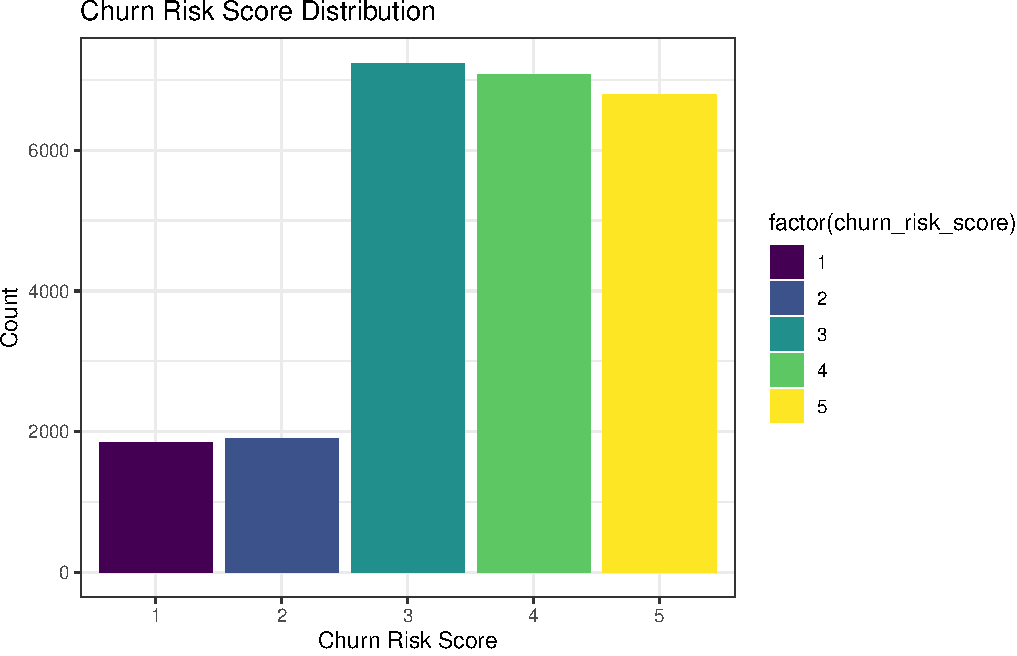
\includegraphics{FPCP4_files/figure-pdf/unnamed-chunk-13-1.pdf}
\end{center}

\begin{center}
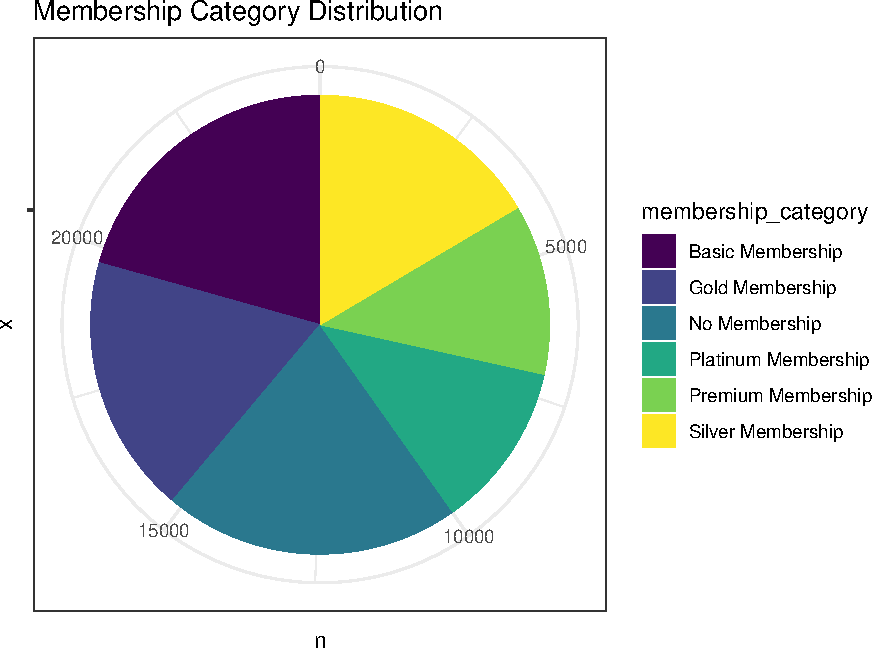
\includegraphics{FPCP4_files/figure-pdf/unnamed-chunk-14-1.pdf}
\end{center}

\begin{center}
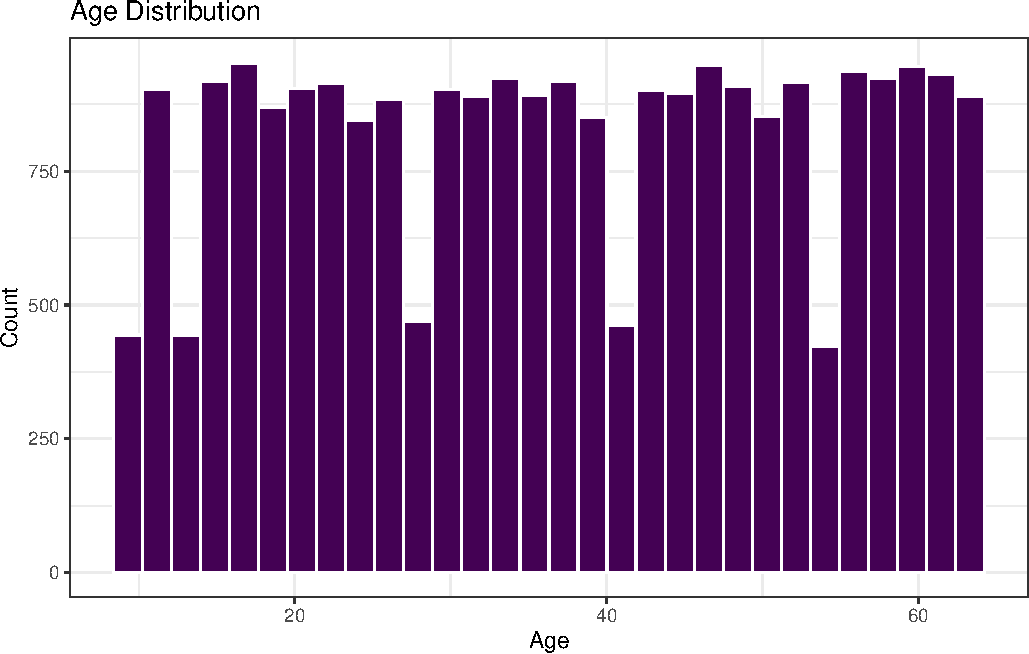
\includegraphics{FPCP4_files/figure-pdf/unnamed-chunk-15-1.pdf}
\end{center}

\begin{center}
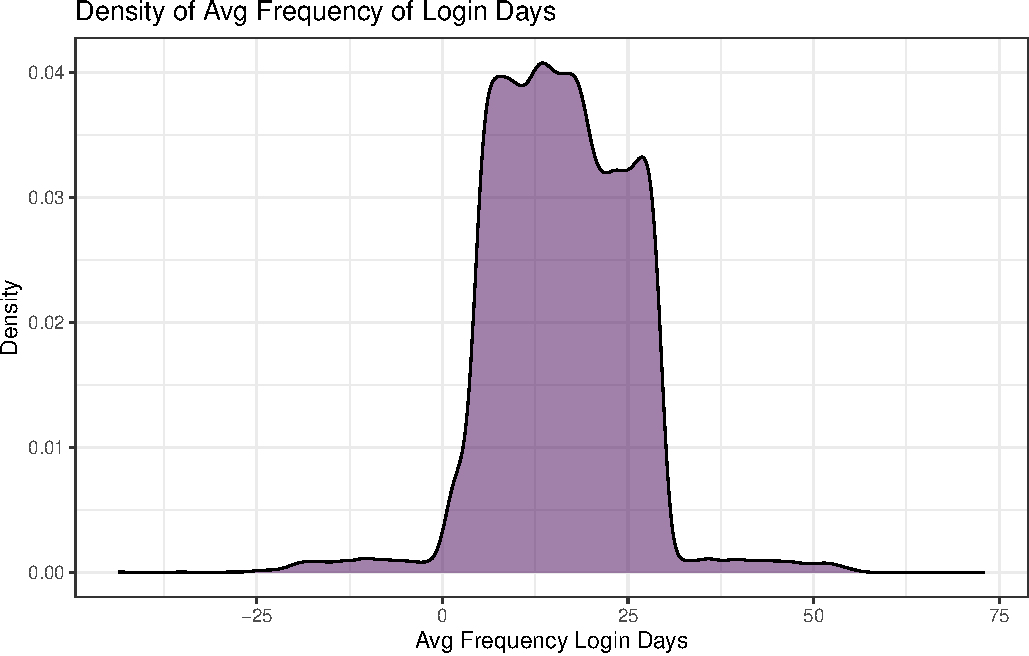
\includegraphics{FPCP4_files/figure-pdf/unnamed-chunk-16-1.pdf}
\end{center}

\begin{center}
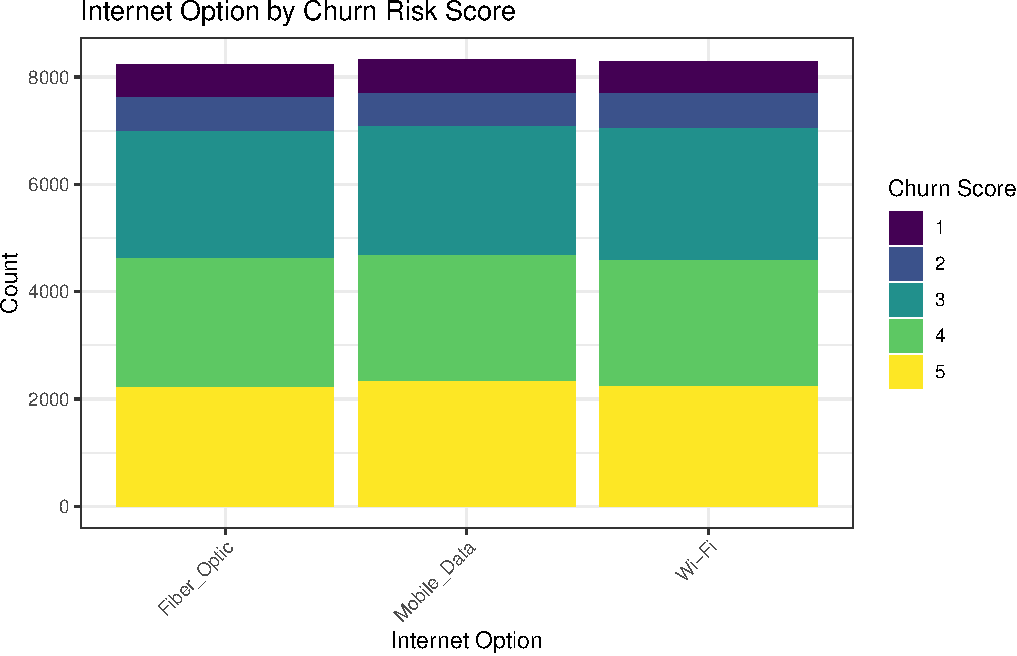
\includegraphics{FPCP4_files/figure-pdf/unnamed-chunk-17-1.pdf}
\end{center}

\begin{center}
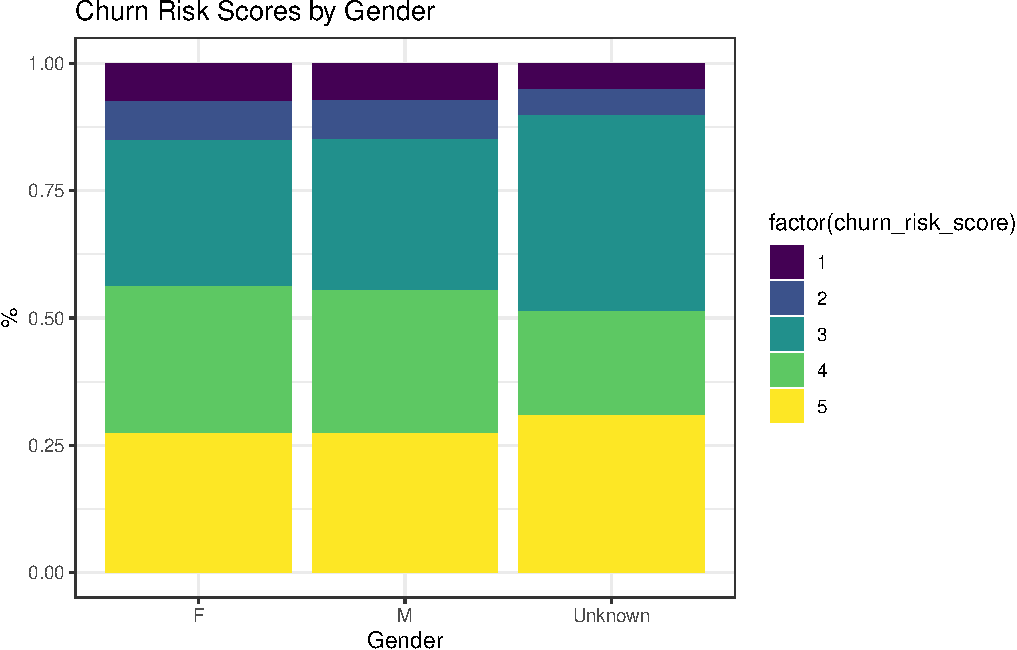
\includegraphics{FPCP4_files/figure-pdf/unnamed-chunk-18-1.pdf}
\end{center}

\begin{center}
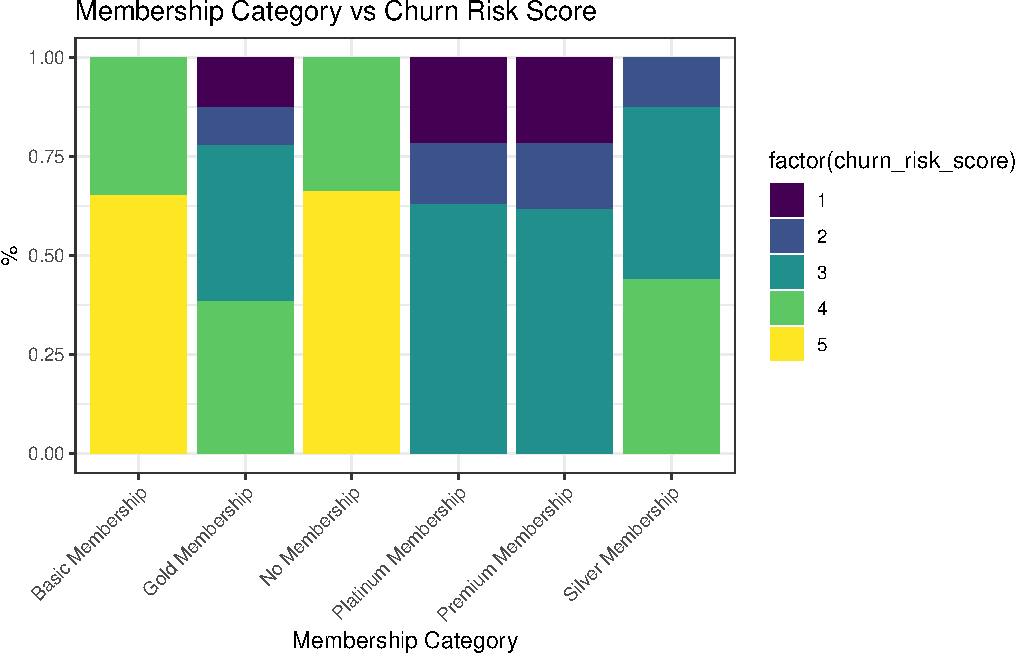
\includegraphics{FPCP4_files/figure-pdf/unnamed-chunk-19-1.pdf}
\end{center}

\begin{center}
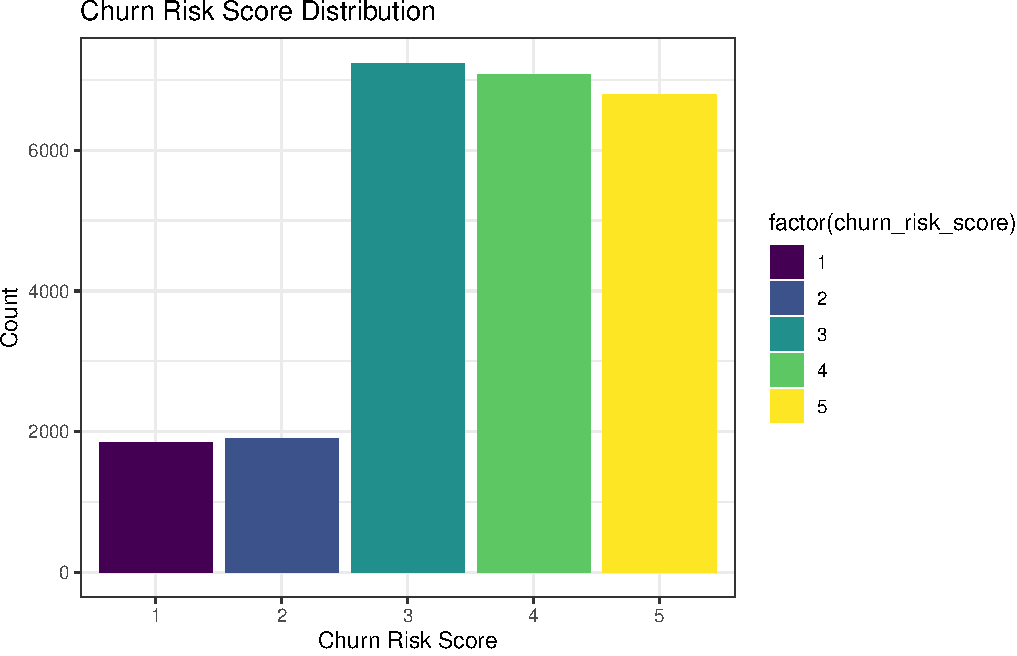
\includegraphics{FPCP4_files/figure-pdf/unnamed-chunk-20-1.pdf}
\end{center}

\begin{center}
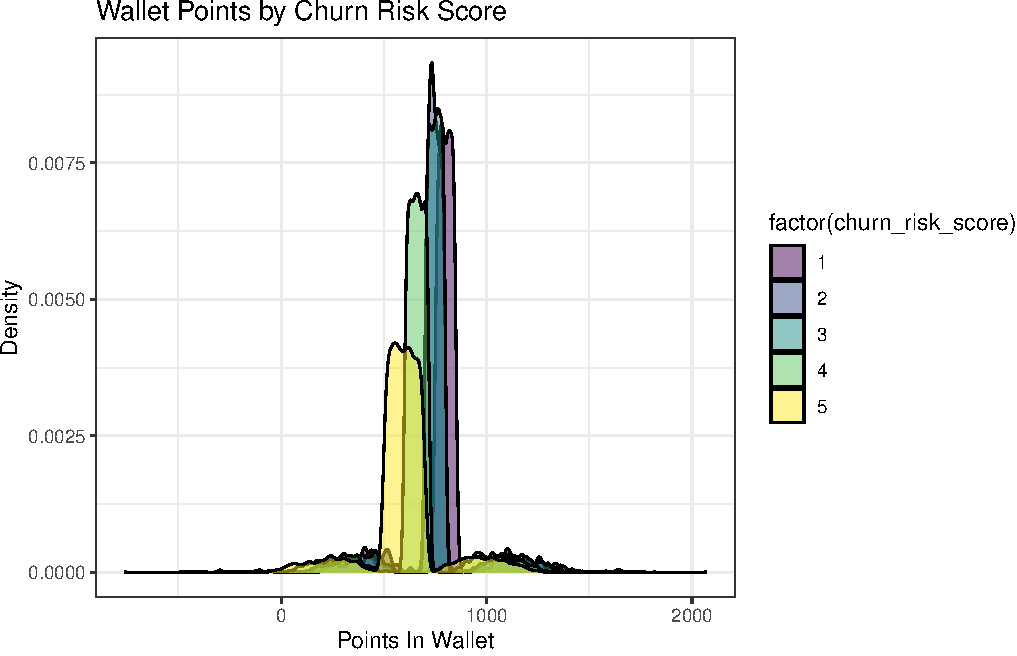
\includegraphics{FPCP4_files/figure-pdf/unnamed-chunk-21-1.pdf}
\end{center}

\begin{center}
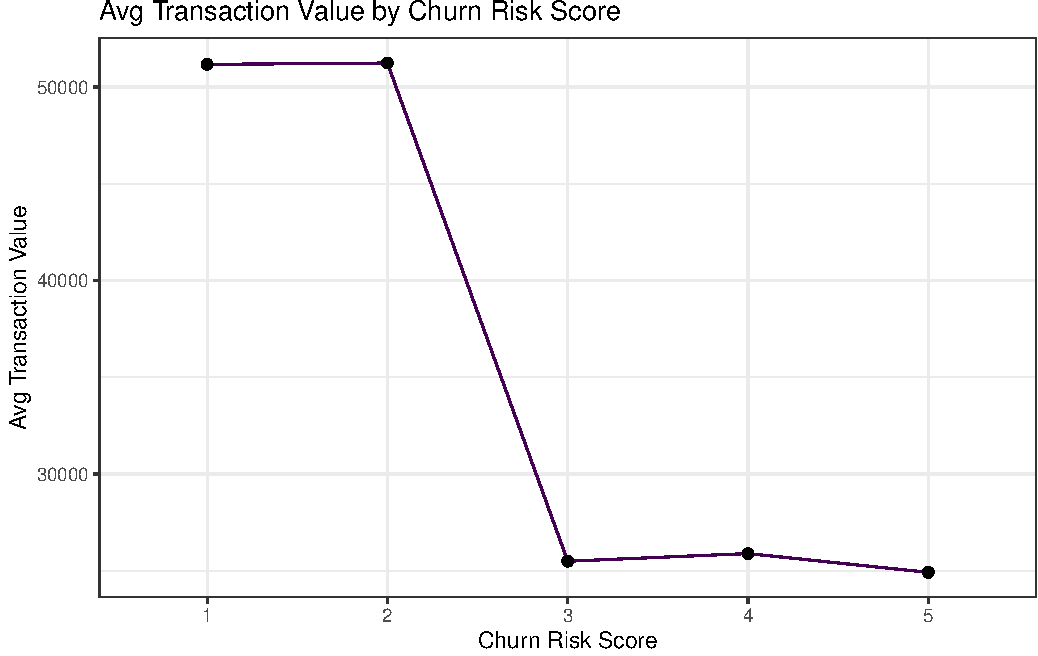
\includegraphics{FPCP4_files/figure-pdf/unnamed-chunk-22-1.pdf}
\end{center}

\begin{center}
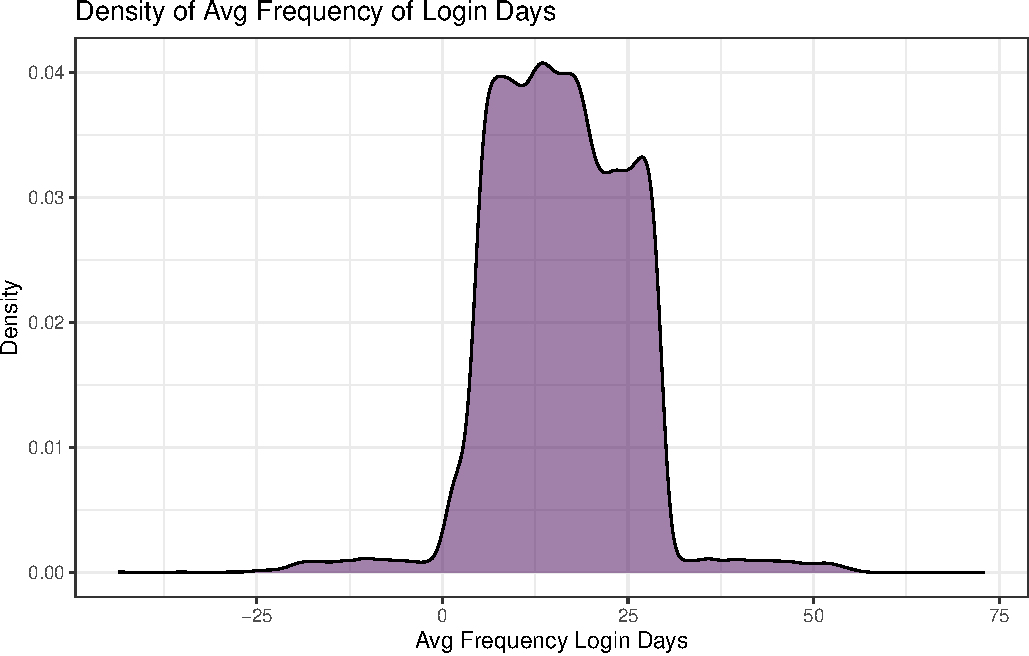
\includegraphics{FPCP4_files/figure-pdf/unnamed-chunk-23-1.pdf}
\end{center}

\section{Modeling Methods}\label{modeling-methods}

\subsection{Linear Regression for Average Transaction
Value}\label{linear-regression-for-average-transaction-value}

We implemented three linear regression models to predict each customer's
average transaction value using different sets of predictors, including
demographic characteristics, engagement behaviors, and their
interactions. Model performance was evaluated using 10-fold
cross-validation with mean absolute error (MAE) as the primary metric.

Model 1 includes basic demographic and membership info to see if certain
types of customers are more likely to churn.

\begin{Shaded}
\begin{Highlighting}[]
\NormalTok{model\_1 }\OtherTok{\textless{}{-}}\NormalTok{ lm\_spec }\SpecialCharTok{\%\textgreater{}\%} \FunctionTok{fit}\NormalTok{(avg\_transaction\_value }\SpecialCharTok{\textasciitilde{}}\NormalTok{ age }\SpecialCharTok{+}\NormalTok{ gender }\SpecialCharTok{+}\NormalTok{ region\_category }\SpecialCharTok{+}\NormalTok{ membership\_category, }\AttributeTok{data =}\NormalTok{ data)}
\end{Highlighting}
\end{Shaded}

Model 2 focuses on recent customer behavior, since more active users may
have lower churn risk.

\begin{Shaded}
\begin{Highlighting}[]
\NormalTok{model\_2 }\OtherTok{\textless{}{-}}\NormalTok{ lm\_spec }\SpecialCharTok{\%\textgreater{}\%} \FunctionTok{fit}\NormalTok{(avg\_transaction\_value }\SpecialCharTok{\textasciitilde{}}\NormalTok{ avg\_time\_spent }\SpecialCharTok{+}\NormalTok{ avg\_frequency\_login\_days }\SpecialCharTok{+}\NormalTok{ days\_since\_last\_login }\SpecialCharTok{+}\NormalTok{ points\_in\_wallet, }\AttributeTok{data =}\NormalTok{ data)}
\end{Highlighting}
\end{Shaded}

Model 3 combines features from all domains and includes interaction
between age and gender.

\begin{Shaded}
\begin{Highlighting}[]
\NormalTok{model\_3 }\OtherTok{\textless{}{-}}\NormalTok{ lm\_spec }\SpecialCharTok{\%\textgreater{}\%} \FunctionTok{fit}\NormalTok{(avg\_transaction\_value }\SpecialCharTok{\textasciitilde{}}\NormalTok{ age}\SpecialCharTok{*}\NormalTok{gender }\SpecialCharTok{+}\NormalTok{ avg\_time\_spent }\SpecialCharTok{+}\NormalTok{ membership\_category }\SpecialCharTok{+}\NormalTok{ past\_complaint }\SpecialCharTok{+}\NormalTok{ internet\_option }\SpecialCharTok{+}\NormalTok{ points\_in\_wallet, }\AttributeTok{data =}\NormalTok{ data)}
\end{Highlighting}
\end{Shaded}

\begin{Shaded}
\begin{Highlighting}[]
\NormalTok{mae\_1\_in}
\end{Highlighting}
\end{Shaded}

\begin{verbatim}
# A tibble: 1 x 3
  .metric .estimator .estimate
  <chr>   <chr>          <dbl>
1 mae     standard      15093.
\end{verbatim}

\begin{Shaded}
\begin{Highlighting}[]
\NormalTok{mae\_2\_in}
\end{Highlighting}
\end{Shaded}

\begin{verbatim}
# A tibble: 1 x 3
  .metric .estimator .estimate
  <chr>   <chr>          <dbl>
1 mae     standard      15139.
\end{verbatim}

\begin{Shaded}
\begin{Highlighting}[]
\NormalTok{mae\_3\_in}
\end{Highlighting}
\end{Shaded}

\begin{verbatim}
# A tibble: 1 x 3
  .metric .estimator .estimate
  <chr>   <chr>          <dbl>
1 mae     standard      15089.
\end{verbatim}

\begin{Shaded}
\begin{Highlighting}[]
\CommentTok{\# 10{-}fold CV MAE}
\NormalTok{cv\_1 }\OtherTok{\textless{}{-}}\NormalTok{ model\_1\_cv }\SpecialCharTok{\%\textgreater{}\%} \FunctionTok{collect\_metrics}\NormalTok{() }\SpecialCharTok{\%\textgreater{}\%} \FunctionTok{filter}\NormalTok{(.metric }\SpecialCharTok{==} \StringTok{"mae"}\NormalTok{)}
\NormalTok{cv\_2 }\OtherTok{\textless{}{-}}\NormalTok{ model\_2\_cv }\SpecialCharTok{\%\textgreater{}\%} \FunctionTok{collect\_metrics}\NormalTok{() }\SpecialCharTok{\%\textgreater{}\%} \FunctionTok{filter}\NormalTok{(.metric }\SpecialCharTok{==} \StringTok{"mae"}\NormalTok{)}
\NormalTok{cv\_3 }\OtherTok{\textless{}{-}}\NormalTok{ model\_3\_cv }\SpecialCharTok{\%\textgreater{}\%} \FunctionTok{collect\_metrics}\NormalTok{() }\SpecialCharTok{\%\textgreater{}\%} \FunctionTok{filter}\NormalTok{(.metric }\SpecialCharTok{==} \StringTok{"mae"}\NormalTok{)}
\end{Highlighting}
\end{Shaded}

\begin{Shaded}
\begin{Highlighting}[]
\CommentTok{\# 10{-}fold CV MAE}
\NormalTok{cv\_1 }
\end{Highlighting}
\end{Shaded}

\begin{verbatim}
# A tibble: 1 x 6
  .metric .estimator   mean     n std_err .config             
  <chr>   <chr>       <dbl> <int>   <dbl> <chr>               
1 mae     standard   15100.    10    55.2 Preprocessor1_Model1
\end{verbatim}

\begin{Shaded}
\begin{Highlighting}[]
\NormalTok{cv\_2 }
\end{Highlighting}
\end{Shaded}

\begin{verbatim}
# A tibble: 1 x 6
  .metric .estimator   mean     n std_err .config             
  <chr>   <chr>       <dbl> <int>   <dbl> <chr>               
1 mae     standard   15142.    10    83.5 Preprocessor1_Model1
\end{verbatim}

\begin{Shaded}
\begin{Highlighting}[]
\NormalTok{cv\_3 }
\end{Highlighting}
\end{Shaded}

\begin{verbatim}
# A tibble: 1 x 6
  .metric .estimator   mean     n std_err .config             
  <chr>   <chr>       <dbl> <int>   <dbl> <chr>               
1 mae     standard   15099.    10    81.9 Preprocessor1_Model1
\end{verbatim}

\begin{longtable}[]{@{}lrr@{}}
\toprule\noalign{}
Model & IN-SAMPLE MAE & 10-fold CV MAE \\
\midrule\noalign{}
\endhead
\bottomrule\noalign{}
\endlastfoot
\texttt{model\_1} & 15092.84 & 15100.21 \\
\texttt{model\_2} & 15138.97 & 15141.82 \\
\texttt{model\_3} & 15088.64 & 15098.81 \\
\end{longtable}

We selected the following linear model based on the lowest
cross-validation error:

\begin{align*}
\text{avg\_transaction\_value}_i &= \beta_0 
+ \beta_1 \cdot \text{age}_i 
+ \beta_2 \cdot \text{gender}_i 
+ \beta_3 \cdot (\text{age}_i \times \text{gender}_i) \\
&+ \beta_4 \cdot \text{avg\_time\_spent}_i 
+ \beta_5 \cdot \text{membership\_category}_i 
+ \beta_6 \cdot \text{past\_complaint}_i \\
&+ \beta_7 \cdot \text{internet\_option}_i 
+ \beta_8 \cdot \text{points\_in\_wallet}_i 
+ \varepsilon_i
\end{align*}

\begin{Shaded}
\begin{Highlighting}[]
\NormalTok{model\_3\_coefs }\OtherTok{\textless{}{-}} \FunctionTok{tidy}\NormalTok{(model\_3)}

\FunctionTok{library}\NormalTok{(kableExtra)}

\NormalTok{model\_3\_coefs }\SpecialCharTok{\%\textgreater{}\%}
  \FunctionTok{kable}\NormalTok{(}\AttributeTok{digits =} \DecValTok{5}\NormalTok{, }\AttributeTok{caption =} \StringTok{"Estimated Coefficients for Final Linear Model"}\NormalTok{) }\SpecialCharTok{\%\textgreater{}\%}
  \FunctionTok{kable\_styling}\NormalTok{(}\AttributeTok{full\_width =} \ConstantTok{FALSE}\NormalTok{)}
\end{Highlighting}
\end{Shaded}

\begin{table}

\caption{Estimated Coefficients for Final Linear Model}
\centering
\begin{tabular}[t]{l|r|r|r|r}
\hline
term & estimate & std.error & statistic & p.value\\
\hline
(Intercept) & 23154.20927 & 679.00320 & 34.10029 & 0.00000\\
\hline
age & -3.30417 & 10.72318 & -0.30813 & 0.75798\\
\hline
genderM & 39.89084 & 614.04528 & 0.06496 & 0.94820\\
\hline
genderUnknown & -2327.08737 & 8235.67046 & -0.28256 & 0.77751\\
\hline
avg\_time\_spent & 0.89741 & 0.30396 & 2.95244 & 0.00316\\
\hline
membership\_categoryGold Membership & 5499.32097 & 394.44063 & 13.94208 & 0.00000\\
\hline
membership\_categoryNo Membership & 62.73415 & 375.28374 & 0.16716 & 0.86724\\
\hline
membership\_categoryPlatinum Membership & 9694.10077 & 451.36484 & 21.47731 & 0.00000\\
\hline
membership\_categoryPremium Membership & 9668.61909 & 447.52127 & 21.60483 & 0.00000\\
\hline
membership\_categorySilver Membership & 3170.06113 & 404.17922 & 7.84321 & 0.00000\\
\hline
past\_complaintYes & -285.87934 & 241.95659 & -1.18153 & 0.23740\\
\hline
internet\_optionMobile\_Data & -7.60142 & 296.40771 & -0.02565 & 0.97954\\
\hline
internet\_optionWi-Fi & -279.77984 & 296.66931 & -0.94307 & 0.34565\\
\hline
points\_in\_wallet & 3.48218 & 0.64709 & 5.38130 & 0.00000\\
\hline
age:genderM & 3.19497 & 15.21981 & 0.20992 & 0.83373\\
\hline
age:genderUnknown & 38.63170 & 188.91160 & 0.20450 & 0.83797\\
\hline
\end{tabular}
\end{table}

Among all predictors, average time spent on the platform and points in
wallet were significantly and positively associated with average
transaction value. Specifically, each additional unit of time spent is
associated with an increase of approximately \$0.90, and each additional
point in the wallet corresponds to an increase of \$3.48 in transaction
value.

Membership category was also a strong predictor. Compared to the
baseline group (Basic Membership), customers with Gold, Platinum,
Premium, and Silver memberships had significantly higher average
transaction values, with coefficients ranging from approximately \$3,170
(Silver) to \$9,694 (Platinum).

In contrast, demographic variables such as age, gender, and their
interaction terms were not statistically significant. Behavioral and
engagement factors might be more informative predictors of customer
spending than demographics in this context.

\subsection{Logistic Regression for High Churn
Risk}\label{logistic-regression-for-high-churn-risk}

We model the churn risk e using the following predictors:

\begin{itemize}
  \item \texttt{age}
  \item \texttt{gender}
  \item \texttt{points\_in\_wallet}
  \item \texttt{avg\_time\_spent}
  \item \texttt{membership\_category}
\end{itemize}

We model the log-odds of being high churn risk (\(Y = 1\)) as:

\[
\log\left( \frac{\mathbb{P}(Y = 1 \mid X_1, \ldots, X_5)}{1 - \mathbb{P}(Y = 1 \mid X_1, \ldots, X_5)} \right)
= \beta_0 + \beta_1 \cdot \mathrm{age} + \beta_2 \cdot \mathrm{gender} +
\beta_3 \cdot \mathrm{points\_in\_wallet} + \beta_4 \cdot \mathrm{avg\_time\_spent} +
\beta_5 \cdot \mathrm{membership\_category}
\]

\begin{Shaded}
\begin{Highlighting}[]
\NormalTok{logit\_model }\OtherTok{\textless{}{-}} \FunctionTok{glm}\NormalTok{(}
\NormalTok{  churn\_high }\SpecialCharTok{\textasciitilde{}}\NormalTok{ age }\SpecialCharTok{+}\NormalTok{ gender }\SpecialCharTok{+}\NormalTok{ points\_in\_wallet }\SpecialCharTok{+}\NormalTok{ avg\_time\_spent }\SpecialCharTok{+}\NormalTok{ membership\_category, }\AttributeTok{data =}\NormalTok{ data, }\AttributeTok{family =} \FunctionTok{binomial}\NormalTok{(}\AttributeTok{link =} \StringTok{"logit"}\NormalTok{)}
\NormalTok{)}
\end{Highlighting}
\end{Shaded}

\begin{Shaded}
\begin{Highlighting}[]
\FunctionTok{summary}\NormalTok{(logit\_model)}
\end{Highlighting}
\end{Shaded}

\begin{verbatim}

Call:
glm(formula = churn_high ~ age + gender + points_in_wallet + 
    avg_time_spent + membership_category, family = binomial(link = "logit"), 
    data = data)

Deviance Residuals: 
     Min        1Q    Median        3Q       Max  
-2.51978  -0.00005   0.00004   0.00005   2.61243  

Coefficients:
                                         Estimate Std. Error z value Pr(>|z|)
(Intercept)                             2.280e+01  2.403e+02   0.095    0.924
age                                     2.242e-03  1.414e-03   1.586    0.113
genderM                                -6.778e-02  4.538e-02  -1.494    0.135
genderUnknown                          -1.009e+00  7.886e-01  -1.279    0.201
points_in_wallet                       -3.336e-03  1.552e-04 -21.493   <2e-16
avg_time_spent                         -2.809e-05  5.744e-05  -0.489    0.625
membership_categoryGold Membership     -2.093e+01  2.403e+02  -0.087    0.931
membership_categoryNo Membership       -2.234e-02  3.391e+02   0.000    1.000
membership_categoryPlatinum Membership -4.103e+01  4.009e+02  -0.102    0.918
membership_categoryPremium Membership  -4.106e+01  3.972e+02  -0.103    0.918
membership_categorySilver Membership   -2.071e+01  2.403e+02  -0.086    0.931
                                          
(Intercept)                               
age                                       
genderM                                   
genderUnknown                             
points_in_wallet                       ***
avg_time_spent                            
membership_categoryGold Membership        
membership_categoryNo Membership          
membership_categoryPlatinum Membership    
membership_categoryPremium Membership     
membership_categorySilver Membership      
---
Signif. codes:  0 '***' 0.001 '**' 0.01 '*' 0.05 '.' 0.1 ' ' 1

(Dispersion parameter for binomial family taken to be 1)

    Null deviance: 34118  on 24852  degrees of freedom
Residual deviance: 11056  on 24842  degrees of freedom
AIC: 11078

Number of Fisher Scoring iterations: 19
\end{verbatim}

Based on the results, we can observe that from this data context:

\begin{itemize}
\item
  age: For each 1-year increase in age, the odds of high churn risk
  increase slightly.
\item
  genderMale: Being male is associated with slightly lower odds of high
  churn risk compared to being female.
\item
  genderUnknown: Having unknown gender is associated with much lower
  odds of high churn risk compared to being female.
\item
  points\_in\_wallet: For each additional point in the wallet, the odds
  of high churn risk decrease slightly.
\item
  avg\_time\_spent: For each additional unit of average time spent, the
  odds of high churn risk decrease very slightly.
\item
  Gold Membership: Being a Gold member is associated with very low odds
  of high churn risk compared to Basic.
\item
  No Membership: Having no membership is associated with little to no
  change in churn risk compared to Basic.
\item
  Platinum Membership: Being a Platinum member is associated with very
  low odds of high churn risk compared to Basic.
\item
  Premium Membership: Being a Premium member is associated with very low
  odds of high churn risk compared to Basic.
\item
  Silver Membership: Being a Silver member is associated with very low
  odds of high churn risk compared to Basic.
\end{itemize}

Since \textbf{points in wallet} appeared to be a significant predictor
of churn risk, we provide a more detailed interpretation of its effect.
The estimated coefficient was

\[
\hat{\beta}_{\mathrm{points\_in\_wallet}} = -0.003336
\]

\begin{Shaded}
\begin{Highlighting}[]
\FunctionTok{exp}\NormalTok{(}\SpecialCharTok{{-}}\FloatTok{0.003336}\NormalTok{)}
\end{Highlighting}
\end{Shaded}

\begin{verbatim}
[1] 0.9966696
\end{verbatim}

We found that each additional point in the wallet \textbf{reduces the
odds of being high churn risk by about 0.33\%}. We also simulated
predictions for representative customers from our dataset.

\begin{Shaded}
\begin{Highlighting}[]
\NormalTok{new\_data }\OtherTok{\textless{}{-}} \FunctionTok{data.frame}\NormalTok{(}
  \AttributeTok{age =} \FunctionTok{c}\NormalTok{(}\DecValTok{25}\NormalTok{, }\DecValTok{45}\NormalTok{),}
  \AttributeTok{gender =} \FunctionTok{factor}\NormalTok{(}\FunctionTok{c}\NormalTok{(}\StringTok{"F"}\NormalTok{, }\StringTok{"M"}\NormalTok{), }\AttributeTok{levels =} \FunctionTok{levels}\NormalTok{(data}\SpecialCharTok{$}\NormalTok{gender)),}
  \AttributeTok{points\_in\_wallet =} \FunctionTok{c}\NormalTok{(}\DecValTok{100}\NormalTok{, }\DecValTok{300}\NormalTok{),}
  \AttributeTok{avg\_time\_spent =} \FunctionTok{c}\NormalTok{(}\DecValTok{20}\NormalTok{, }\DecValTok{5}\NormalTok{),}
  \AttributeTok{membership\_category =} \FunctionTok{factor}\NormalTok{(}\FunctionTok{c}\NormalTok{(}\StringTok{"Basic Membership"}\NormalTok{, }\StringTok{"Gold Membership"}\NormalTok{),}
                               \AttributeTok{levels =} \FunctionTok{levels}\NormalTok{(data}\SpecialCharTok{$}\NormalTok{membership\_category))}
\NormalTok{)}

\NormalTok{predicted\_probs }\OtherTok{\textless{}{-}} \FunctionTok{predict}\NormalTok{(logit\_model, }\AttributeTok{newdata =}\NormalTok{ new\_data, }\AttributeTok{type =} \StringTok{"response"}\NormalTok{)}

\FunctionTok{cbind}\NormalTok{(new\_data, }\AttributeTok{predicted\_probability =}\NormalTok{ predicted\_probs)}
\end{Highlighting}
\end{Shaded}

\begin{verbatim}
  age gender points_in_wallet avg_time_spent membership_category
1  25      F              100             20    Basic Membership
2  45      M              300              5     Gold Membership
  predicted_probability
1             1.0000000
2             0.7120415
\end{verbatim}

From our data context, we could predict that a 25-year-old female with
100 wallet points, 20 average time spent, and Basic Membership has a
predicted probability of 1 of being high churn risk. On the other hand,
a 45-year-old male with 300 wallet points, 5 average time spent, and
Gold Membership has a predicted probability of 0.712 of being high churn
risk.

It is worth noting that logistic regression is better suited for binary
outcomes because it ensures predicted probabilities stay between 0 and
1, while linear regression can produce invalid probabilities outside
that range. Logistic regression models the log-odds, but its
coefficients are more difficult to interpret.

\section{Conclusion}\label{conclusion}

This project applied linear regression to predict average transaction
value and logistic regression to classify high churn risk. Results
indicated that behavioral features, such as time spent on the platform
and points in wallet, were more predictive than demographic variables.
Cross-validation was used to compare model performance, and the final
models highlighted key factors associated with customer spending and
retention. Overall, the analysis suggests that more engaged users tend
to spend more and are less likely to churn.




\end{document}
